\documentclass{article}
\usepackage{cite}
\usepackage{amsmath,amssymb,amsfonts}
\usepackage{algorithm, algorithmic}
\usepackage{graphicx}
\usepackage{textcomp}
\usepackage{xcolor}
\def\BibTeX{{\rm B\kern-.05em{\sc i\kern-.025em b}\kern-.08em
    T\kern-.1667em\lower.7ex\hbox{E}\kern-.125emX}}
\graphicspath{ {./results/plots/} }


\title{Dynamic Portfolio Rebalancing with ADP}

\author{1\textsuperscript{st} John-Craig Borman
\textit{School of Business} \\
\textit{Stevens Institute of Technology}\\
Hoboken, New Jersey \\
jborman@stevens.edu
\and
{2\textsuperscript{nd} Somayeh Moazeni
\textit{School of Business} \\
\textit{Stevens Institute of Technology}\\
Hoboken, New Jersey \\
smoazeni@stevens.edu}
}

\begin{document}

\newcommand{\ssep}{:}

\maketitle

\begin{abstract}
Portfolio rebalancing is a widely studied practice both in the investment industry and academia. Commonly, heuristic methods are used to provide ad-hoc sub-optimal decision signals to trigger rebalancings. Dynamic programming methods, however, provide optimal solutions as well as robust and flexible frameworks which may be specialized to meet the specific needs of an investor.
We investigate the practical application of dynamic programming methodologies to the portfolio rebalancing problem starting with a generally accepted framework and then further developing this model to better reflect the peculiarities of non-normal financial data.
\end{abstract}


Keywords: dynamic programming, value iteration, portfolio rebalancing, portfolio management, transaction costs


\section{Introduction}

\subsection{Overview}

This paper seeks to implement a robust and systematic solution to the portfolio rebalancing problem using approximate dynamic programming on stochastic processes. 

\subsection{Practical Importance}

Quite simply, anyone who invests money in assets, either directly or indirectly, owns a portfolio. Portfolios, like their underlying assets, have risk and return characteristics that evolve over time. The focus of portfolio rebalancing is then to help the investor successfully navigate a portfolio across market regimes towards a particular risk/return based objective. 

The importance of asset allocation has been a frequently discussed topic in both the academic and professional investing communities. Most notably \cite{b3} identified that asset allocation explains 95\% of the variation in total pension plan returns between 1974-83. Beyond academia, Vanguard Group has been a preeminent voice in the professional community advocating for rebalancing as a means of reducing a portfolio's drift away from its initial asset allocation. "Portfolio drift" can result in the development of undesirable risk-return characteristics over time \cite{b1}. The registered investment advisor suggests that "investors’ focus should be on the asset allocation choice and its implementation using broadly diversified, low-cost portfolios with limited market-timing" \cite{b4}.

While asset allocation has its own area of research on identifying the optimal portfolio, rebalancing strategies seek to maintain the risk-return characteristics of the optimal allocation while minimizing the costs of doing so.

\subsection{Rebalancing Strategies}

Rebalancing strategies generally fall within two categories: fixed and random time.

\paragraph{Fixed Time} Commonly referred to as periodic methods, these strategies rebalance at fixed time intervals typically of the quarterly, semi-annual or annual frequencies, regardless of the magnitude of drift. Higher frequency intervals can produce higher transaction costs as a rebalancing can be unnecessary when the portfolio has drifted little from its optimal allocation \cite{b1} \cite{b5}. Meanwhile, lower frequency rebalancings may suffer from increased drift and an undesirable allocation. 

Another set of strategies known as threshold methods instead rebalance only when a portfolio, tracking its optimal allocation, has exceeded a specified tracking error. However, threshold rebalancing strategies are still evaluated at fixed points in time. Empirical results demonstrate that combinations of 'time-and-threshold' strategies help minimize rebalancing costs as well as limit portfolio drift \cite{b1}.

\paragraph{Random Time} Both previously mentioned fixed time methods fall under the category of heuristics. Instead of rebalancing because it is an optimal decision for the portfolio, the decision to rebalance occurs due to a signal. Random time strategies, however, derive an optimal decision from the current asset allocation. That is, the decision on whether to rebalance or not is calculated based on the current state and the likelihood of transitioning to different allocations at future points in time. 

\subsection{The Model} The model in this paper is grounded in the work of Sun et al.'s "Optimal Rebalancing for Institutional Portfolios" \cite{b5}. We begin with their dynamic programming framework solving the Bellman equation by applying a finite time horizon value iteration method. Using this result as the baseline, we demonstrate a number of improvements by departing from their assumptions that a). asset returns are normally distributed following a multiplicative dynamic model and b). mean and variance are the statistical moments of interest.

\subsection{Empirical Results}

\subsection{Organization} The organization of the paper is as follows. In Section II we layout the formal mathematics and notation behind our model as well as the improvements to \cite{b5}. Section III will expand upon the methodology of the experiment and how the results are to be evaluated. Section IV details the computational results and analytics of a basic two asset scenario and that applied to the sector ETFs of the S\&P 500. Section V will close the paper, summarize and conclude on the results. 

\section{The Model}

The mathematical framework follows that of a classic dynamic programming model using a Bellman equation to express the present value of expected future cost. The model is presented from the ground up starting with the object and notation, then further developing the model to fully express the portfolio rebalancing problem. 

\subsection{Objective}

The objective of the portfolio rebalancing problem is to make a decision to rebalance or not while minimizing the cost sustained by the portfolio. The cost of rebalancing a portfolio is typically described by the transaction costs incurred when assets are bought and sold in order to obtain a desired allocation. However, \cite{b5} recognizes that a portfolio also suffers costs when in a suboptimal allocation such that an investor is not meeting their risk-return objectives. \cite{b5} uses the difference in certainty-equivalent returns between two portfolios as a model for sub-optimality costs. Their method allows for transaction costs and sub-optimality costs to be described in the same units of return and can therefore be minimized together.

The objective of this dynamic programming problem is then to minimize current and future expected costs. In doing so, the evaluation of this model provides a cost-informed decision to a portfolio manager on whether or not the current asset allocation should be rebalanced solely based on information derived from the state of the portfolio.

\subsection{Notation}

\subsubsection{State Variable}
A portfolio can simply be described as a vector of weights $w$ containing elements $w_i$ representing the proportional cash allocation to asset $i$. For the sake of simplicity we will restrict short selling and leveraging such that the state space of possible portfolios can be described by: 
\begin{equation}
W = \{w \in \mathbb{R}^n \ssep \sum_{i = 1}^{n} w_i = 1,  w_i \in [0, 1] \} \label{eq:state-space}
\end{equation}
While a portfolio's state may change over time, the state space remains constant.

\subsubsection{Decision Variable}
The portfolio's state can change as a result of two exogenous factors, the first being stochastic changes in the underlying asset values and the second being a portfolio manager's explicit decision to purchase and sell assets. The stochastic changes are represented by the random variable $\eta$ while the deliberate changes in asset allocation are expressed by $u$. Thus, the next portfolio state at time $t+1$ can be represented by some function of the current state variable and the two aforementioned exogenous variables representing changes to the state: 
\begin{equation}
w_{t+1} = H(w_t, u_t, \eta_t) \label{eq:state-transition}
\end{equation}
where $u_t$ is the decision variable in the set $U$ described as:

\begin{equation}
u_t \in U = \{u_t \in \mathbb{R}^n \ssep u_t + w_t = w_{t+1} \forall w_t, w_{t+1} \in W\} \label{eq:decision-space}
\end{equation}

\subsubsection{Transition Probabilities}
For any two portfolios we can describe the probability that the portfolio will transition from an initial state $w$ to $w'$ as the probability of the weight change in each asset occurring together. Let the vector of weight changes between the two states be described by $$\Delta w = w' - w$$ such that the transition probability function $$\mathbb{P}: $$ 
\begin{equation}
\mathbb{P}(w'|w) = \mathbb{P}(\Delta w) = \prod_{i = 0}^{n}\mathbb{P}(\Delta w_i) \label{eq:transition-prob}
\end{equation}
Note that the transition probability model above does not assume any particular distribution and can be built upon with models that better reflect the particular probabilistic nature of asset returns in the market.

\subsubsection{Cost Functions}
As mentioned previously, the cost of being in state $w_t$ can be broken down into two components representing transaction costs and sub-optimality costs. Using the same notation as \cite{b5}, transaction costs will be described by the function $\tau(w_t, u_t)$ while sub-optimality costs will be represented by the function $\epsilon(w_t, w_{t+1})$. Let the cost function $G$ be written as:
\begin{equation}
G(w_t, u_t, \eta_t) = \tau(w_t, u_t) + \epsilon(w_t, w_{t+1}). \label{eq:cost-fun1}
\end{equation}
or using equation \ref{eq:state-transition} expressing $w_{t+1}$ as a function:
\begin{equation}
G(w_t, u_t, \eta_t) = \tau(w_t, u_t) + \epsilon(w_t,  H(w_t, u_t, \eta_t)) \label{eq:cost-fun2}
\end{equation}

\subsubsection{Bellman Equation}
Now to connect the previous notation with a recursive Bellman equation, let the function $J_t(w_t)$ represent the sum of the current expected cost $G$ plus the expected cost at the next time step $J_{t+1}(w_{t+1})$:
\begin{equation}
J_t(w_t) = \mathbb{E}[G(w_t, u_t, \eta_t) + \gamma J_{t+1}(w_{t+1})] \label{eq:bellman}
\end{equation}
where $\gamma$ is a discount factor. Since future costs carry less weight that the current costs to be incurred, future $J_t$ values should be discounted. The result is that as $t$ approaches some horizon $T$ the $\lim\limits_{t \to T}{J_t = 0}$. This is true for sufficiently large $T$ and requires that $\gamma \in (0, 1)$. 

The objective of the model is to minimize the total expected cost $J_t$ such that the optimal cost is minimized with respect to our decision variable $u_t$:
\begin{equation}
J_t^*(w_t) = \min_{u_t \in U} \mathbb{E}[G(w_t, u_t, \eta_t) + \gamma J_{t+1}(w_{t+1})] \label{eq:bellman-opt}
\end{equation}

In order to convert the expectation in equations \ref{eq:bellman} and \ref{eq:bellman-opt} to a deterministic problem, we can apply the transition probability model from equation  \ref{eq:transition-prob} so that:

\begin{equation}
J_t(w_t) = \sum_{w' \in W} \mathbb{P}(w' | w) \times [G(w_t, u_t, \eta_t) + \gamma J_{t+1}(w')] \label{eq:bellman-det}
\end{equation}

and 

\begin{equation}
J_t^*(w_t) = \min_{u_t \in U} \sum_{w' \in W} \mathbb{P}(w' | w) \times [G(w_t, u_t, \eta_t) + \gamma J_{t+1}(w')] \label{eq:bellman-opt-det}
\end{equation}

\section{Methodology}

With the formal mathematics laid out, the following subsections described the current assumptions made in order to make the problem computationally tractable.

\subsection{Computational Framework}

We will first assume that, as a portfolio manager, we have the option to rebalance our portfolio only at the end of a trading day. Thus the manager may only ever observe the state variable $w$ at discrete points in time $t$. The stochastic changes in asset weights from the market $\eta_t$ then occur between end of day close-to-close points in time. If $w_t$ is the current allocation today, then $w_t + u_t$ is the allocation post-rebalancing today and $\eta_t$ are the stochastic weight fluctuations incurred during the next intra-day market activity. The function $H$ in equation \ref{eq:state-transition} being a simple additive dynamic model is represented by:

\begin{equation}
w_{t+1} = H(w_t, u_t, \eta_t) = (w_t + u_t) + \eta_t
\end{equation}

Since the previous assumption recognizes discrete realizations of $w$ and $u$, the stochastic changes $\eta$ must lay in some set $E$ containing discretized weight changes incremented by $l$ such that: 
\begin{equation}
 E = \{l\delta \ssep w_{min} \leq w_i \pm l\delta \leq w_{max}, l \in [w_{min}, w_{max}], \delta = D(\sigma)  \}
\end{equation}
Where $w_{min}$ and $w_{max}$ are the minimum and maximum possible weight allocations to any single asset, $l$ is the atomic weight increment, and $D(\sigma )$ is a discretized normal distribution function.
\begin{equation}
 D(\sigma) = nint(N(0, \sigma)) \label{eq:normal-discretized}
\end{equation}
Here, $nint: \mathbb{R} \to \mathbb{I}$ is an arbitrary nearest integer function. The state space in equation \ref{eq:state-space} can then be restated in a discretized form:
\begin{equation}
W = \{w \in \mathbb{R} \ssep \sum_{i = 1}^{n} w_i = 1,  w_i + \eta \in [w_{min}, w_{max}], \forall \eta \in E \} \label{eq:state-space2}
\end{equation}
and $\mathbb{P}: \mathbb{I} \to [0, 1]$ is a probability density function that maps an integer back to a discretized normal probability. 

\subsection{Parameters and Tests}

The dynamic programming equation will be solved over a finite time horizon of $T = 240$ using value iteration. It will be assumed that $J_T(w) = 0, \forall w \in W$. Then stepping backward and solving for $J_t$ at each $t \in \{T, T-1, ..., 2, 1, 0\}$. Starting with a 3 asset portfolio consisting of the S\&P 500 sector ETFs XLK,  XLF and XLE and the optimal allocation as the equal weight portfolio of $\begin{bmatrix} 0.33 && 0.33 && 0.34 \end{bmatrix}$, respectively. 

\subsection{Algorithm}

The algorithm below was developed to implement the aforementioned computational framework using value iteration as the solution method:

\begin{algorithm}
\caption{Calculate $J_t(w_t) \forall w_t \in W, t \in \{0, 1, ..., T\}$}
\label{al:value-iteration}
\begin{algorithmic}
	\STATE Let $w_{init} \in W$ be the initial allocation
	\STATE $T = 240, \gamma = 0.9$      
	\STATE $J_T(w_T) = 0, \forall w_T \in W$ 
	\FOR{$t = T-1$ \TO $0$}
		\STATE $J_t(w_t) = \infty, \forall w_t \in W$ 
		\FOR{$i = 1$ \TO $|W|$}
			\STATE $J_t(w_i) = \sum_{w' \in W} \mathbb{P}(w' | w_i) \times [G(w_i, u_t, \eta_t) + \gamma J_{t+1}(w')]$
		\ENDFOR
	\ENDFOR	
	\STATE $J_0^*(w^*) = \min_{w \in W} J_0(w)$
	\STATE $u_0^* = w^* - w_{init}$
	\RETURN $u_0^*$
\end{algorithmic}
\end{algorithm}

\section{Computational Results}

When the optimal weight is set to the equal weight portfolio allocation, the visualization of a 3 asset state space colorized by the $J_0(w_0)$ values is show in Figure \ref{fig:optimal-space}.

\subsection{Improvements (temporary subsection)}

\paragraph{Note} This is a temporary subsection to acknowledge measures to improve the current process as well as any highlight any known errors in the preceding work.

\paragraph{Code} At the moment the expectation is being improperly calculated such that the probability of being in some future state $w_{t+1}$ is not being applied to the corresponding expected future cost values. Instead $J_{t+1}$ is solely being discounted by $gamma$ and then added to the expected value of the current cost $G$. See Figure \ref{fig:code-error1} for the current implementation.

\begin{figure}
	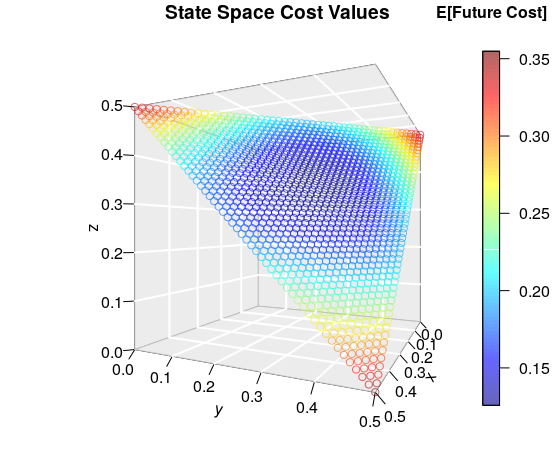
\includegraphics[width=\textwidth]{Optimal-Weight-Plot-v2.png} 	
	\caption{Discretized state space of expected future cost values at t = 0}
	\label{fig:optimal-space} 
\end{figure}

\begin{figure}
	\centering
	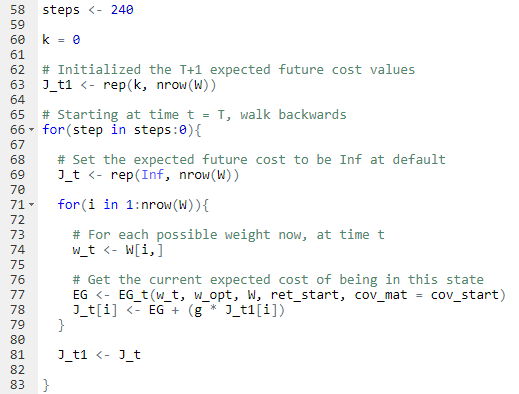
\includegraphics[width=9cm, height=8cm]{results/plots/code-error1}
	\caption{Current algorithm implemented in R}
	\label{fig:code-error1}
\end{figure}
 

\section{Conclusion}

\section*{References}

Unless there are six authors or more give all authors' names; do not use 
``et al.''. Papers that have not been published, even if they have been 
submitted for publication, should be cited as ``unpublished'' \cite{b4}. Papers 
that have been accepted for publication should be cited as ``in press'' \cite{b5}. 
Capitalize only the first word in a paper title, except for proper nouns and 
element symbols.

\begin{thebibliography}{00}
\bibitem{b1} Jaconetti, Colleen M, et al. Best Practices for Portfolio Rebalancing. Vangaurd, July 2010.
\bibitem{b2} Pula, Justina \& Berisha, Gentrit \& Ahmeti, Skender. (2012). The Impact of Portfolio Diversification in the Performance and the Risk of Investments of Kosovo Pension Savings Trust. Journal of Business and Economics. 3. 198-211. 10.15341/jbe(2155-7950)/03.03.2012/005. 
\bibitem{b3} Brinson, Gary P., L. Randolph Hood, and Gilbert L. Beebower, 1986. Determinants of Portfolio Performance. Financial Analysts Journal 42(4): 39–48.
\bibitem{b4} Davis, Joseph H, et al. The Asset Allocation Debate: Provocative Questions, Enduring Realities. 2007, The Asset Allocation Debate: Provocative Questions, Enduring Realities.
\bibitem{b5} Sun, Walter, et al. “Optimal Rebalancing for Institutional Portfolios.” Journal of Portfolio Management, vol. 32, no. 2, 2006, pp. 33–43., doi:https://doi.org/10.3905/jpm.2006.611801.

\end{thebibliography}

\end{document}
